\chapter{Discriminante Lineal de Fisher}
\label{ch:chapter2}

En este capítulo se hablará del Análisis Discriminante Lineal de Fisher (ADLF), el cual busca optimizar un cociente de la forma $Tr(V^T A V) / Tr(V^T B V)$ sobre el conjunto de matrices ortogonales $V$ con $A, B$ matrices positivas definidas. Para resolver el ADLF, se han presentado en libros de aprendizaje estadístico y clasificación de patrones formulaciones alternas al problema original, ya que este era considerado computacionalmente muy costoso \cite{wang2007trace}\cite{ngo2012trace}. Planteamientos como: maximizar la traza de la matriz de dispersión entre clases sujeto a una restricción sobre la matriz de dispersión interna, maximizar la traza del cociente de matrices; o bien, maximizar el cociente de determinantes, han sido formulaciones presentadas en distintos textos \cite{duda2012pattern} \cite{hastie2009elements} \cite{mitchell2006discipline} \cite{fukunaga2013introduction}. Al final, todas estas propuestas resultan ser versiones simplificadas del problema.

En este capítulo se resolverá el problema original del ADLF a través del método de Newton-Lanczos, el cual resulta ser computacionalmente eficiente. En la primer sección del capítulo se contextualizará al problema dentro del área de Aprendizaje de Máquina. En la segunda parte, se proporcionará la teoría correspondiente para seguir con facilidad el texto. Por último, en la tercera parte, se plantea la solución al problema de ADLF para una dimensión, se generaliza a $p$ dimensiones y se proporcionan las condiciones para la existencia de la solución.


\section{Aprendizaje de máquina}
El Aprendizaje de Máquina toma como base dos áreas de investigación: la Ciencia de la Computación y la Estadística. De la primera, retoma las preguntas: ¿Cómo se pueden construir máquinas que resuelvan problemas? Y ¿Qué problemas son tratables o intratables? De la segunda, toma las preguntas: ¿Qué puede ser inferido de los datos? ¿Bajo que supuestos del modelo? Y ¿Con qué confiabilidad? \cite{mitchell2006discipline}. El esfuerzo por resolver estas preguntas da como resultado una disciplina enfocada a construir teorías estadístico-computacional de los procesos de aprendizaje.

\subsection{Procesos de aprendizaje}

Se dice que una máquina ``aprende" dada una tarea (T), una medición del rendimiento (R) y un tipo de experiencia (E) si el sistema mejora confiablemente su rendimiento (R) en la tarea (T) dada la experiencia (E) \cite{mitchell2006discipline}. Es decir, se modela una estructura con los datos proporcionados de manera que el rendimiento en la tarea mejora conforme más información recibe. La diversidad de las tareas, así como el campo de aplicaciones es muy diverso, por ejemplo:

\begin{itemize} 

\item \textit{Clasificación de spam/no-spam}, en el que (E) son los correos, (T) el clasificar correctamente el \textit{spam} y (R) el porcentaje de correos correctamente clasificados.

\item \textit{Reconocimiento/Clasificación facial}, en el que (E) son los rostros de distintas personas, (T) el reconocimiento o clasificación de los rostros y (R) el porcentaje de rostros correctamente reconocidos o clasificados.
\end{itemize} 

Los procesos de aprendizaje tienen diversas aplicaciones y distintos supuestos, por lo que han surgido clasificaciones para analizarlos en conjunto. La utilizada en este texto es la propuesta por T. Hastie \cite{hastie2009elements}, la cual divide a los métodos en dos grupos: aprendizaje supervisado y aprendizaje no supervisado. El primero, supone la presencia de una variable de salida que actúa como guía en la construcción de la estructura. Ejemplos de éste es la regresión lineal, los árboles de decisión y las máquinas de soporte vectorial. 
Por otra parte, el aprendizaje no supervisado solo cuenta con la información de las variables independientes; por ejemplo, análisis de conglomerados, reglas de asociación y reducción dimensional. 

Después de esta primer clasificación, se subclasifica a los métodos de aprendizaje supervisado de acuerdo al tipo de variable de salida (Figura 1.1). \footnote{A lo largo del texto se usará indiferentemente variable de entrada como ``input'' o variable independiente y variable de salida como ``output'' o variable dependiente} Cuando se trata de una variable cuantitativa recibe el nombre de regresión, mientras que en el caso de cualitativas se le llama clasificación. Por otra parte, el aprendizaje no supervisado tiene dos ramas en las que el texto hace énfasis \cite{hastie2009elements}: Segmentación en el caso que se desee asignar un grupo a cada individuo, de manera que los grupos sean homogéneos entre sí; o bien, reducción dimensional cuando solamente se desea proyectar a los individuos en un espacio de menor dimensión, de manera que se cumplan características especiales en dicho subespacio. 

El problema de ADLF pertenece a la rama de aprendizaje supervisado, en particular a los métodos clasificación. Alternativas para esta finalidad, y que sigan asumiento linealidad en la frontera, son la Regresión Logística, el Análisis Discriminante Lineal y las Máquinas de Soporte Vectorial. 

\begin{figure}[!ht]
  \centering
  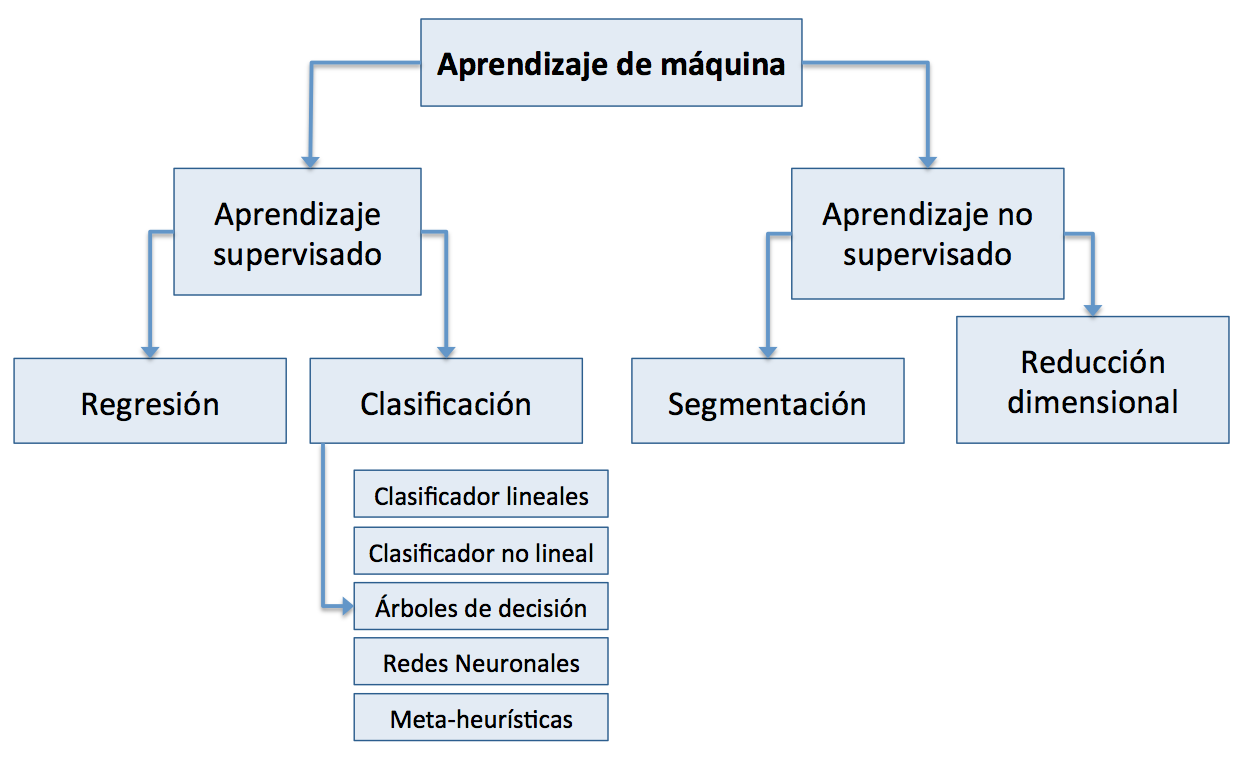
\includegraphics[width=1\textwidth]{Figures/Chapter1_Clasificacion1.png} 
  \caption[Enfoques para resolver problemas de clasificación.]
  {Distintos enfoques para resolver problemas de clasificación en el área de Aprendizaje de Máquina.}
\end{figure}

\section{Matrices de dispersión}
Se comenzará definiendo la nomenclatura necesaria para la sección. Sea $x_i$ el individuo $i$ que pertenece a la clase $y_i$, $N_{k}$ el número de personas en la clase $k$, $N$ el número total de personas y $w_i = V^T x_i$; es decir, los datos proyectados con la matriz $V$. Entonces, se definen las medias de grupo $k$ como $\mu_k$ y la media de todos los datos $x_i$ como $\mu$:

\begin{equation} \label{eq:18}
  \mu_k = \frac{1}{N_{k}} 
  \sum_{\substack{i = 1\\
                    y_i = k}}^{N}
                  x_i
\end{equation} 

\begin{equation} \label{eq:19}
 \mu = \frac{1}{N} \sum_{i = 1}^{N} x_i
\end{equation}

Por otro lado, se definen las medias correspondientes a los datos proyectados $w_i$:
\begin{equation} \label{eq:20}
  \widetilde{\mu_k} = \frac{1}{N_{k}} 
  \sum_{\substack{i = 1\\
                    y_i = k}}^{N}
                  w_i
\end{equation} 

\begin{equation} \label{eq:21}
 \widetilde{\mu} = \frac{1}{N} \sum_{i = 1}^{N} w_i
\end{equation}

El ADLF hace amplio uso de las matrices de dispersión, en específico de la matriz de covarianza, la matriz de dispersión de todos los individuos, la matriz de dispersión interna y la matriz de dispersión entre clases. Es importante analizar a profundidad la terminología y las fórmulas que se usarán a lo largo de la tesis para entender la lógica detrás de la formulación.

Sea $\Sigma$ la matriz de covarianza (\textit{Covariance Matrix)} de todos los individuos. Se define como $\widehat{\Sigma}$ al estimador insesgado de $\Sigma$ el cual está escalada entre $N-1$:

\begin{equation} \label{eq:2.1}
\widehat{\Sigma} = \frac{1}{N-1} \sum_{i=1}^{N}(x_i - \mu)(x_i - \mu)^T	
\end{equation}

Si esta matriz no está escalada por $N-1$ entonces se le conoce como matriz de dispersión (\textit{Scatter Matrix}), en esta tesis se representará como $S_T$, con el subíndice $T$ que significa que está tomando en cuenta a todos los individuos:

\begin{equation} \label{eq:2.2}
S_T = \sum_{i=1}^{N}(x_i - \mu)(x_i - \mu)^T	
\end{equation}

Cuando solo se toman a los individuos de una clase particular $k$, se puede encontrar su correspondiente matriz de dispersión, representada como $S_k$, con el subíndice $k$ simbolizando que está tomando en cuenta solo a los individuos de la clase $k$:

\begin{equation*}
S_k = \sum_{\substack{i=1 \\ y_i = k}}^{N} (x_k - \mu)(x_k - \mu)^T	
\end{equation*}

De esta manera se define la matriz de dispersión interna (\textit{Within-class scatter matrix}) como la suma sobre $k$ de todas las matrices de dispersión de cada clase:

\begin{equation}\label{eq:2.3}
S_I = \sum_{k=1}^{K} 
					\sum_{\substack{i = 1\\
                  			   	y_i = k}}
                    ^{N}
 ({x_i-\mu_{k}})({x_i-\mu_{k}})^T 	
\end{equation}

Ahora solo falta definir la matriz de dispersión entre clases (\textit{Between-class scatter matrix}) como la suma de diferencias al cuadrado de las medias de clase contra la media de todos los datos multiplicada por el número de individuos en cada clase $N_k$:

\begin{equation} \label{eq:2.4}
S_E = \sum_{k = 1}^K N_k (\mu_k - \mu)(\mu_k - \mu)^T	
\end{equation}

\begin{figure}[!ht] \label{Fig1.1}
  \centering
	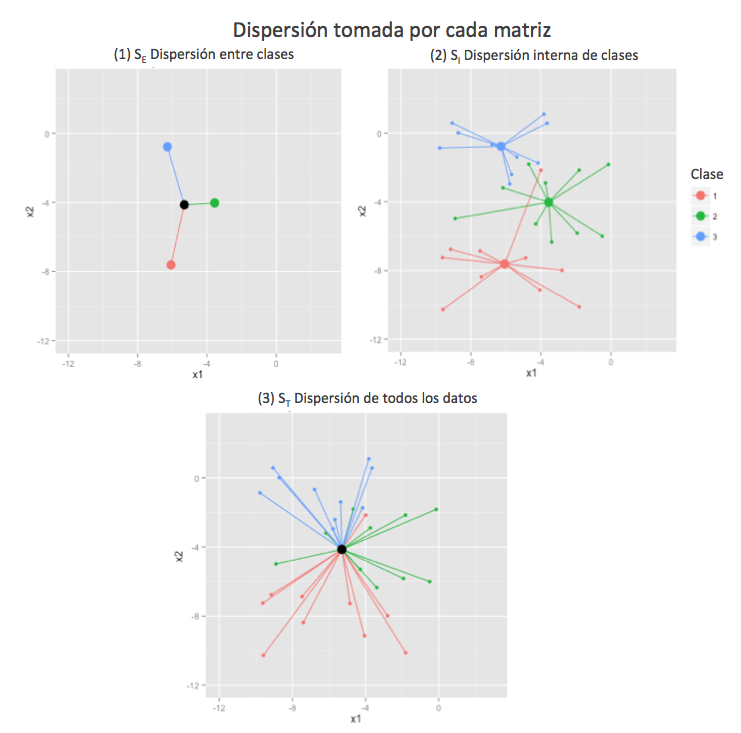
\includegraphics[width=1\textwidth]{Figures/Chapter2_SE_SI}	
  \caption[Distancias en las matrices de dispersión.]
  {En la gráfica (1) se representa la $S_E$, es decir las distancias al cuadrado entre la media de todos los datos (Punto negro) y las medias de cada clase (Puntos de color gruesos). La gráfica (2) representa $S_I$; es decir, la distancia al cuadrado de los individuos a la media de su clase. La gráfica (3) representa $S_T$, la dispersión de los datos con respecto a la media de todos.}
\end{figure}

Entre la matriz de dispersión interna $S_I$, la matriz de dispersión entre clases $S_E$ y la matriz de dispersión total $S_T$ existe una relación importante. Se cumple que $S_T = S_I + S_E $; es decir, la dispersión de las medias de grupos con la media global más la dispersión de cada clase individual es igual a la dispersión de los datos sin la información de las clases. Los datos de la figura 1.2 representan las distancias que toman en cuenta cada una de estas matrices. Para ejemplificar esta relación se generaron 10 datos por clase suponiendo distribuciones normales (El coeficiente de correlación de los datos generados es $-0.005$):

\begin{center}
\begin{tabular}{ c c c}
\toprule
\textbf{Clase} & \textbf{Distribución x1} & \textbf{Distribución x2} \\
\midrule\\
\addlinespace[-2ex]
1 & N(-5, 2.5) & N(-8, 2)\\
2 & N(-3, 2.5) & N(-4, 2)\\
3 & N(-7, 2.5) & N(-1, 2) \\
\addlinespace[1.5ex]
\bottomrule
\end{tabular}
\end{center}

Calculando las matrices de dispersión de acuerdo a las fórmulas (1.6), (1.7) y (1.8):

\begin{center}
\begin{tabular}{ c c c}
\toprule
\textbf{$S_I$} & \textbf{$S_E$} & \textbf{$S_T$} \\
\midrule\\
\addlinespace[-2ex]
$ \begin{bmatrix}  186.05 & 2.78 \\ 2.78 &  94.58 \end{bmatrix}$ &
$ \begin{bmatrix} 46.13 & -4.15 \\ -4.15 & 234.57 \end{bmatrix}$ &
$ \begin{bmatrix}  232.18 & -1.36 \\ -1.36 &  329.16 \end{bmatrix}$ \\
\addlinespace[1.5ex]
\bottomrule
\end{tabular}
\end{center}

De este ejemplo numérico se puede ver que al sumar la dispersión interna $S_I$ y la dispersión entre clases $S_E$ da como resultado la dispersión de todos los individuos $S_T$. En general este resultado se cumple, por lo que a continuación se enuncia esta relación que es muy fácil de demostrar.

\begin{proposition} \label{lemma2.1}
Sea $S_E$ la matriz de dispersión entre clases, $S_I$ la matriz de dispersión interna y $S_T$ la matriz de dispersión de los datos, entonces se tiene que cumplir la siguiente igualdad: $S_T$ = $S_I$ + $S_E$
\end{proposition}

Un problema muy común que surge en problemas de aprendizaje estadístico es que el costo computacional puede volverse intratable conforme la dimensionalidad de los individuos crece. En el ADLF se requiere hacer el cómputo de las matrices de dispersión de los individuos constantemente (o bien calcular la inversa de matrices de alta dimensionalidad), cálculos que para grandes dimensiones son sumamente costosos. Existen distintas maneras para hacer frente a este problema, uno de ellos involucra el PCA (Principal Component Analysis) en el preprocesamiento de los datos. Este método es fácil de calcular y solo requiere computar una vez la de matriz de dispersión \cite{ngo2012trace}. Debido a la finalidad de esta tesis no se profundizará en más técnicas para hacer frente a este problema, pero en textos como \cite{hastie2009elements}, \cite{duda2012pattern} aparecen distintos métodos para reducción de dimensionalidad.

Retomando el problema de cociente de trazas, lo que se busca es encontrar la proyección que mantenga juntos individuos de una clase al mismo tiempo que separa las medias de distintas clases. Una vez obtenida esta proyección se puede encontrar un hiperplano separador de los datos, o bien algún criterio para asignar la clase de pertenencia. 

\pagebreak
El problema de optimización se puede plantear como:
\begin{equation}\label{eq:2.5}
	\max_{\substack{V \in {\rm I\!R}^{n \times p} \\ V^TC V = I}} \frac{Tr(V^T S_E V)}{Tr(V^T S_I V)} 	
\end{equation}

 La solución a este problema no tiene una forma cerrada, por lo que en la literatura se buscan formulaciones alternas para resolverlo de una manera más sencilla \cite{wang2007trace} \cite{fukunaga2013introduction}, algunos ejemplos de estas formulaciones son:

\begin{equation}\label{eq:2.6}
	\max_{\substack{V \in {\rm I\!R}^{n \times p} \\ V^T S_I V = I}} Tr(V^T S_E V)
\end{equation}

\begin{equation} \label{eq:2.7}
	\max_{\substack{V \in {\rm I\!R}^{n \times p} \\ V^TC V = I}} Tr\left( \frac{V^T S_E V}{V^T S_I V}\right) 	
\end{equation}

\begin{equation} \label{eq:2.8}
	\max_{\substack{V \in {\rm I\!R}^{n \times p} \\ V^TC V = I}} \frac{|V^T S_E V|}{|V^T S_I V|} 	
\end{equation}

Con $|\bullet| = det(\bullet)$ y $Tr(\bullet) = Traza(\bullet)$.


En la siguiente parte de este capítulo se resolverá el problema original (1.9) para $p = 1$, para lo cual se introduce el cociente generalizado de Rayleigh. Para la generalización a $p$ dimensiones solo se plantea el problema y se proporcionan los casos en que la solución existe y es única. Seguido de esto se definirá una función $f(\rho)$ la cual sirve para encontrar el óptimo por métodos iterativos. Por último haciendo uso de los eigenvalores de $S_I$ y $S_E$ se darán cotas inferiores y superiores al óptimo.

\section{Problema del cociente de trazas}

El problema del cociente de trazas (Trace ratio problem) es fácil de ver cuando $V \in {\rm I\!R}^{n \times p}$ proyecta a un espacio de pocas dimensiones. Por ejemplo, cuando $p = 2$ se desea obtener la mejor proyección sobre un plano y cuando $p = 1$ sobre una recta. Para ejemplificar esta situación se creo un conjunto sintético donde cada $x_i \in {\rm I\!R}^{3}$. Las distribuciones son normales y se proyectan en ${\rm I\!R}^{2}$ y ${\rm I\!R}^{1}$. Los datos se pueden observar en la figura 1.3.

\begin{figure}[!ht]\label{Fig1.2}
  \centering
  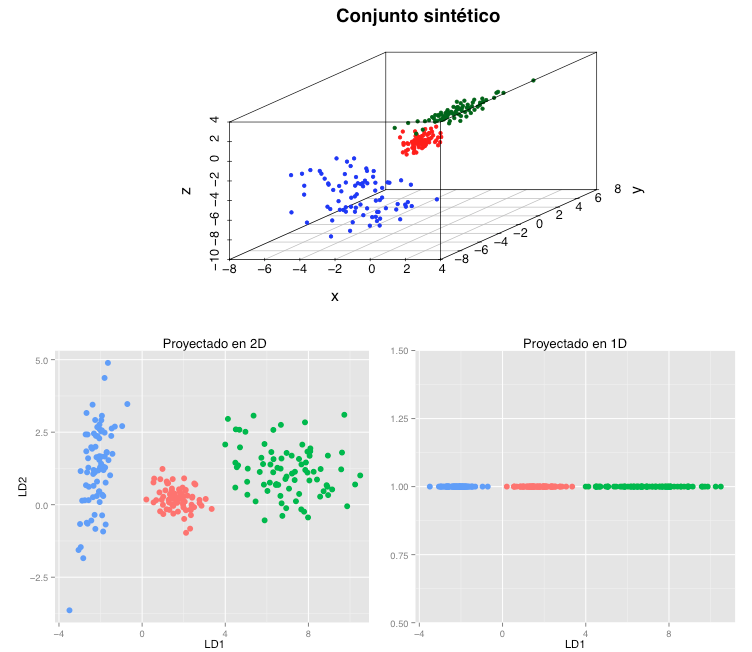
\includegraphics[width=1\textwidth]{Figures/Chapter2_1} 
  \caption[Mejores proyecciones en ${\rm I\!R}^{2}$ y ${\rm I\!R}$.]
  {En la gráfica de arriba se muestran los datos originales en 
   ${\rm I\!R}^{3}$ los cuales fueron generados a través de distribuciones normales con distintas medias y varianzas. En la gráfica de abajo a la izquierda se muestra la mejor proyección en ${\rm I\!R}^{2}$ y abajo a la derecha la mejor proyección en ${\rm I\!R}$}
\end{figure}

\subsection{Solución cuando p = 1}

El problema (1.9) toma la siguiente forma cuando $V \in {\rm I\!R}^{n}$. Se nombrara $v$ a este proyector de una dimensión ya que resulta ser solo un vector:


\begin{equation} \label{eq:2.9}
\max_{v \in {\rm I\!R}^{n}} \frac{v^T S_E v}{v^T S_I v}  
\end{equation}

Se tiene que $x_i \in {\rm I\!R}^{n}$ son los individuos originales con $i = 1 , ... , N $. Entonces sean $w_i \in {\rm I\!R}$ los individuos proyectados por el vector $v$ de manera que $w_i = v^Tx_i$. De esta manera es conveniente definir $\widehat{\mu}_k = v^T \mu_k$ y $\widehat{\mu} = v^T \mu$ como la media por clase y la media total de los datos proyectados.

\textbf{Matriz de dispersión entre clases $\Phi_{E}$ de los individuos proyectados $w_i$:}

$$\Phi_{E} = \sum\limits_{k =1}^{K} N_k (\widehat{\mu}_k - \widehat{\mu} )^2$$

$$\Phi_{E} = \sum\limits_{k =1}^{K} N_k (v^T \mu_k - v^T \mu)^2$$

$$\Phi_{E} =  \sum\limits_{k =1}^{K} N_k v^T ( \mu_k - \mu )(\mu_k - \mu )^T v $$
Por distributividad en matrices se cumple que $vAv+vBv =  v(A+B)v$, entonces:

\begin{equation}\label{eq:2.10}
\Phi_{E} = v^T \big[ \sum\limits_{k =1}^{K} N_k ( \mu_k - \mu )(\mu_k - \mu )^T \big] v	
\end{equation}

\textbf{Matriz de dispersión intra clase $\Phi_{I}$ de los individuos proyectados $w_i$}:
$$\Phi_{I} = \sum\limits_{k = 1}^{K} \sum\limits_{\substack{i = 1\\
                            y_i = k}}^{N} (w_i - \widehat{\mu}_k)^2 $$

$$\Phi_{I} = \sum\limits_{k = 1}^{K} \sum\limits_{\substack{i = 1\\
                            y_i = k}}^{N} (v_i^T x_i - v_i^T \mu_k)^{2} $$
$$\Phi_{I} =  \sum\limits_{k = 1}^{K} \sum\limits_{\substack{i = 1\\
                            y_i = k}}^{ N} v^T( x_i - \mu_k) ( x_i - \mu_k)^T v  $$

Usando de nuevo la distibutividad de matrices:

\begin{equation}\label{eq:2.11}
\Phi_{I} = v^T \big[ \sum\limits_{k = 1}^{K} \sum\limits_{\substack{i = 1\\
                            y_i = k}}^{ N} ( x_i - \mu_k) ( x_i - \mu_k)^T \big] v	
\end{equation}


 Las fórmulas de $\Phi_{I}$ y $\Phi_{E}$ de los individuos $w_i$ se pueden expresar en función de las matrices de dispersión intra clase y entre clases $S_I$ y $S_E$ de los individuos originales $x_i$. De esta manera:

 $$\Phi_{E} = f(S_E) = v^T S_E v$$
 $$\Phi_{I} = f(S_I) = v^T S_I v$$

Se tiene que $\Phi_{I}, \Phi_{E} \in {\rm I\!R}$, entonces maximizar el cociente $\frac{\Phi_{E}}{\Phi_{I}}$ con respecto a $v$ tiene como resultado una proyección que conserva cerca a los individuos pertenecientes a la misma clase, mientras que aleja a los centros de cada clase. Para el caso de una dimensión se puede encontrar una solución cerrada. La teoría asociada a este problema de maximización esta relacionada con el Cociente Generalizado de Rayleigh, el cual bajo las condiciones enunciadas de este caso, se puede transformar a un Cociente de Rayleight. Usando la proposición 1.2 se puede obtener la solución a este último.

\begin{proposition} \label{lemma2.2}
La solución a la maximización del Cociente de Rayleigh:
$$\max_{v \in {\rm I\!R}^{n} } \frac{v^T A v}{v^Tv} $$
cuando $A$ es simétrica, es obtenida cuando $v$ es el eigenvector asociado al eigenvalor más grande de la matriz $A$.
\end{proposition}


\subsection{Generalización a p dimensiones}

Para dimensiones más grandes de $v$, el Cociente Generalizado de Rayleigh no puede ser escrito en general como el Cociente de Rayleigh, por lo que la solución planteada en el capítulo anterior no es de utilidad. Esto genera la dificultad de no tener una solución cerrada, por lo que se han propuesto métodos iterativos y planteamientos alternos a la solución.

La generalización a $p$ dimensiones implica que los individuos $x_i \in {\rm I\!R}^{n}$ son proyectados ahora por la matriz $V = (V_1 | V_2 | ... |V_p)$, de manera que $w_i = V^T x_i$ con $w_i \in {\rm I\!R}^{p}$ y $V_j \in {\rm I\!R}^{n}$. De esta manera las matrices $\Phi_I$ y $\Phi_E$ se definen como sigue:

\begin{equation*}
\Phi_E = \sum\limits_{k = 1}^{K} N_{k} ||\widehat{\mu}_k - \widehat{\mu}||_2^2
\end{equation*}

\begin{equation*}
\Phi_E = \sum\limits_{k = 1}^{K} N_{k} ||V^T \mu_k - V^T \mu||_2^2
\end{equation*}

\begin{equation*}
\Phi_E = \sum\limits_{k = 1}^{K} N_{k} ||V^T (\mu_k - \mu)||_2^2
\end{equation*}


\begin{equation}\label{eq:2.17}
  \Phi_E = \sum\limits_{k = 1}^{K} N_{k} \big[ (V_1^T (\mu_k - \mu))^2 + (V_2^T (\mu_k - \mu))^2+ ... + (V_p^T (\mu_k - \mu))^2 \big]
\end{equation}

De esta expresión hay que destacar que $V_1^T (\mu_k - \mu)$ es un escalar, ya que $V_1 \in {\rm I\!R}^n$ y $(\mu_k - \mu) \in {\rm I\!R}^{n}$. Otra fórmula equivalente y que es comúnmente usada por sus propiedades algebraicas consiste en la siguiente expresión:

\begin{equation}\label{eq:2.18}
\Phi_E = \sum\limits_{k = 1}^{K} N_{k} Tr \big[ V^T (\mu_k - \mu) (\mu_k - \mu)^T V \big]	
\end{equation}

Para ejemplificarla se toma una clase $k = k_1$.  Al desarrollar $(\bullet) = V^T (\mu_1 - \mu) (\mu_1 - \mu)^T V$ se tiene una matriz en ${\rm I\!R}^{p \times p}$ igual a:


\begin{equation*}
(\bullet)= \left(\!
    \begin{array}{c}
      V_1^T (\mu_1-\mu)\\
      V_2^T (\mu_1-\mu)\\
      \vdots \\
      V_p^T (\mu_1-\mu)
    \end{array}
  \!\right) 
  \left(\!\begin{array}{c}
      (\mu_1-\mu)^T V_1 \quad
      (\mu_1-\mu)^T V_2 \quad
      \hdots \quad
      (\mu_1-\mu)^T V_p
    \end{array}
  \!\right) 
\end{equation*} 

\vspace{5mm}

\begin{equation*}
(\bullet)= \left(\!
    \begin{array}{ccc}
      V_1^T (\mu_1-\mu) (\mu_1-\mu)^T V_1 & \hdots & V_1^T (\mu_1-\mu) (\mu_1-\mu)^T V_p  \\
      V_2^T (\mu_1-\mu) (\mu_1-\mu)^T V_1 & \hdots & V_2^T (\mu_1-\mu) (\mu_1-\mu)^T V_p  \\
      \vdots & \ddots & \vdots\\
      V_p^T (\mu_1-\mu) (\mu_1-\mu)^T V_1 & \hdots & V_p^T (\mu_1-\mu) (\mu_1-\mu)^T V_p
    \end{array}
  \!\right) 
\end{equation*} 

\vspace{5mm}

\begin{equation*}
(\bullet)= \left(\!
    \begin{array}{ccc}
      (V_1^T (\mu_1-\mu))^2 & \hdots & V_1^T (\mu_1-\mu) (\mu_1-\mu)^T V_p \\
       V_2^T (\mu_1-\mu) (\mu_1-\mu)^T V_1  & \hdots & V_2^T (\mu_1-\mu) (\mu_1-\mu)^T V_p  \\
      \vdots & \ddots & \vdots\\
      V_p^T (\mu_1-\mu) (\mu_1-\mu)^T V_1  & \hdots & (V_p^T (\mu_1-\mu))^2
    \end{array}
  \!\right) 
\end{equation*} 

\vspace{5mm}

 Por lo tanto al calcular la traza de la matriz de $p \times p$ desarrollada arriba, se tiene que $Tr(V^T (\mu_1 - \mu) (\mu_1 - \mu)^T V)$ es equivalente a:
 \vspace{3mm}
 \begin{equation*}
Tr(\bullet) = (V_1^T (\mu_1-\mu))^2+ (V_2^T (\mu_1-\mu) )^2 + \hdots + (V_p^T (\mu_1-\mu) )^2
 \end{equation*}

Al generalizar a las $K$ clases y usando la propiedad de linealidad en la traza; es decir, $Tr(A+B) = Tr(A)+Tr(B)$, entonces se puede escribir de la siguiente manera:

\begin{equation*}
\Phi_E = Tr \sum\limits_{k = 1}^{K} N_{k}  \big[ V^T (\mu_k - \mu) (\mu_k - \mu)^T V \big]
\end{equation*}


Esta expresión es equivalente a (1.16). Como paso final se factoriza $V^T$ y $V$ sobre todos los sumandos, lo que nos llevaría a lo siguiente:

\begin{equation*} 
\Phi_E =  Tr (V^T \sum\limits_{k = 1}^{K} N_{k}  \big[(\mu_k - \mu) (\mu_k - \mu)^T \big] V)   
\end{equation*}

o, expresada en términos de $S_E = \sum\limits_{k = 1}^{K} N_{k}  \big[(\mu_k - \mu) (\mu_k - \mu)^T \big]$

\begin{equation}\label{eq:2.19}
\Phi_E =  Tr (V^T S_E V)     
\end{equation}

Similarmente se puede llegar a la formulación de la varianza intra-clase $\Phi_{I}$.
\begin{equation}\label{eq:2.20}
\Phi_{I} =  Tr (V^T S_I V )
\end{equation}



\subsection{Existencia de la solución}

Para demostrar la existencia y unicidad de la solución, las matrices $S_I$ y $S_E$ deben cumplir ciertas características. Sean $A = S_E$ y $B = S_I$, la primer condición que se les impone es que sean positivas definidas. La razón que apoya la restricción está relacionada con la forma de la función a maximizar, que es un cociente. Como $B$ se encuentra en el denominador, se tiene que evitar que $Tr(V^T B V) = 0$, ya que con este valor se indetermina la función objetivo \cite{ngo2012trace}. 

T.T. Ngo propone generalizar el estudio a las matrices positivas semidefinidas. Para esto se deben encontrar los casos en que $Tr(V^T B V)$ toma el valor de $0$. Si se diagonaliza a la matriz $B = Q \Lambda_{B} Q^T$ con $Q$ ortogonal y $\Lambda_{B}$ una matriz diagonal con entradas iguales a los eigenvalores de $B$, entonces:

\begin{equation*}
Tr(\Lambda_{B}) = \lambda_{B_1}+ \lambda_{B_2}+ ... +\lambda_{B_n} \qquad con \qquad \widehat{V} = Q^T V
\end{equation*}



De este modo $\widehat{V} = (\widehat{V}_1 | \widehat{V}_2 | ... | \widehat{V}_p)$ y cada $\widehat{V}_i^T = (\widehat{V}_{i1}, \widehat{V}_{i2}, ..., \widehat{V}_{in})$ es un vector renglón. De esta manera la matriz $\widehat{V}^T$:

\begin{equation*}
\widehat{V}^T = 	
\left(\!
    \begin{array}{c}
      \widehat{V}_1^T\\
      \widehat{V}_2^T\\
      \vdots \\
      \widehat{V}_p^T
    \end{array}
  \!\right)   = 
\left(\!
    \begin{array}{cccc}
      \widehat{V}_{11} & \widehat{V}_{12} & \hdots & \widehat{V}_{1n}\\
      \widehat{V}_{21} & \widehat{V}_{22} & \hdots & \widehat{V}_{2n}\\
      \vdots &  \vdots &\ddots & \vdots\\
      \widehat{V}_{p1} & \widehat{V}_{p2} & \hdots & \widehat{V}_{pn}\\
    \end{array}
  \!\right) 
\end{equation*}

Por lo que la traza que involucra a $B$ tiene la siguiente forma:

\begin{equation*}
Tr(V^T B V) = Tr(V^T Q \Lambda_{B} Q^T V) 	
\end{equation*}

\begin{equation*}
Tr(V^T B V)  = Tr(\widehat{V}^T \Lambda_{B} \widehat{V})
\end{equation*}

\begin{equation*}
V^T B V = 
\left(\!
    \begin{array}{c}
      \widehat{V}_1^T\\
      \widehat{V}_2^T\\
      \vdots \\
      \widehat{V}_p^T
    \end{array}
  \!\right) 
  \left(\!
    \begin{array}{cccc}
      \lambda_{B_1} & 0 & \hdots & 0\\
      0 & \lambda_{B_2} & \hdots & 0\\
      \vdots &  \vdots &\ddots & \vdots\\
      0 & 0 & \hdots & \lambda_{B_n}\\
    \end{array}
  \!\right) 
  \left(\!\begin{array}{c}
      \widehat{V}_1 |
      \widehat{V}_2 |
      \hdots |
      \widehat{V}_p
    \end{array}
  \!\right) 
\end{equation*} 

Desarrollando la multiplicación de matrices, y calculando la traza resulta en los siguientes sumandos:
 
 \begin{equation*}
\begin{aligned}
      Tr(V^T B V) =& \lambda_{B_1} \widehat{V}_{11}^2&  +
                     & \lambda_{B_2} \widehat{V}_{12}^2& +
                     & \hdots& +
                     &\lambda_{B_n} \widehat{V}_{1n}^2& + \\
                     & \lambda_{B_1} \widehat{V}_{21}^2&+
                     & \lambda_{B_2} \widehat{V}_{22}^2& +
                     & \hdots& +
                     &\lambda_{B_n} \widehat{V}_{2n}^2& + \\
                     & \vdots&  
                     & \vdots& 
                     & \vdots& 
                     & \vdots& \\
                     & \lambda_{B_1} \widehat{V}_{p1}^2&+
                     & \lambda_{B_2} \widehat{V}_{p2}^2& +
                     & \hdots& + 
                     & \lambda_{B_n} \widehat{V}_{pn}^2.&  
 \end{aligned}
 \end{equation*}

 Es fácil de ver que la expresión de arriba tiene $p \times n$ sumandos, por lo que se puede expresar en términos de dos sumatorias. La primera de $j=1,...,p$ y la segunda de $i = 1,...n$:

\begin{equation*} 
Tr(V^T B V) = \sum \limits_{j=1}^{p} \sum\limits_{i=1}^{n} \lambda_{B_i} \widehat{V}_{ji}^2
\end{equation*}

\begin{equation}\label{eq:2.21}
Tr(V^T B V) = \sum\limits_{i=1}^{n} \lambda_{B_i} \sum \limits_{j=1}^{p} \widehat{V}_{ji}^2    
\end{equation}

De la última expresión se separa la sumatoria sobre $i$. De esta manera, para cada elemento $i$ se tienen dos factores:

\begin{equation}\label{eq:2.22}
(i) \lambda_{B_i}
\end{equation}

 \begin{equation}\label{eq:2.23}
 (ii) \sum \limits_{j=1}^{p} \widehat{V}_{ji}^2   
 \end{equation}
 

 La idea para que $Tr(V^T B V)$ sea positivo, es que al menos uno de los sumandos sea positivo. Si (1.21) y (1.22) son ambos distintos de cero para al menos una $i$, entonces se cumple esta condición. Esta idea está expresada en el Lema 1.1.

\begin{lemma}\label{lemma2.4}
Sea $B$ positiva semidefinida y $V \in {\rm I\!R}^{n\times p}$. Si $B$ tiene a lo más $p-1$ eigenvalores iguales a $0$, entonces $Tr(V^T B V)  = Tr(\widehat{V}^T \Lambda_{B} \widehat{V}) \neq 0$  para cualquier matriz ortogonal $V$.
\end{lemma}

\begin{proof}
Sea $\widehat{V} = [\widehat{V}_1 | ... | \widehat{V}_p]$ tal que $\widehat{V} \widehat{V} = V^T Q Q^T V = V^T I_n V  = I_p$. De esta manera se puede construir una matriz $\widehat{V}' \in {\rm I\!R}^{p \times p}$ seleccionando $p$ de los $n$ renglones de $\widehat{V}$ tal que $\widehat{V}'$ sea no singular. $\widehat{V}'$ tiene la propiedad de no contener eigenvalores iguales a 0; como consecuencia, sus renglones y columnas no contienen al vector $\widehat{0}$. Al no contenerlo,se sabe que al menos hay $p$ renglones de $\widehat{V}$ tal que $\sum_{j=1}^{p}\widehat{V}_{ji}^2 \neq 0$ para cada uno de ellos. Por otra parte en el lema se supone que la matriz $B$ tiene a lo más $p-1$ eigenvalores iguales $0$ por lo que al menos un elemento de la sumatoria es distinto de cero.
\end{proof}

Analizando a mayor profundidad el resultado anterior, se sabe que hay $n-p+1$ eigenvalores de $B$ positivos ($\lambda_{B_i} \neq 0$) y $p$ renglones de $\widehat{V}$ que tienen norma distinta de cero. Al calcular la sumatoria (1.20), se tiene que al menos una combinación de $\lambda_{B_i}$ y uno de los $p$ renglones cumplen que su multiplicación tiene signo positivo. Para ejemplificar esta situación sean $C_i$ con $i = 1, ... , n-p+1$ los eigenvalores de $B$ y $K_j$ con $j = 1, ... , p$ la norma de los renglones de $\widehat{V}$ que son distintos de $0$.
 
\begin{center}
\begin{tabular}{ | c | c|  c | c|} 
\hline
$i$ & $\lambda_{B_i}$ & $\sum \limits_{j=1}^{p} \widehat{V}_{ji}^2$  & $\lambda_{B_i} \sum \limits_{j=1}^{p} \widehat{V}_{ji}^2$ \\ 
\hline
\hline
1 & $C_1$ & $0$ & $0$ \\ 
\hline
2 & $C_2$ & $0$ & $0$ \\ 
\hline
\vdots & \vdots & \vdots & \vdots \\ 
\hline
$n-p$ & $C_{n-p}$ & $0$ &  $0$\\ 
\hline
$n-p+1$ & $C_{n-p+1}$ & $K_{p}$ &  $C_{n-p+1} K_{p}$\\ 
\hline
$n-p+2$ & $0$ & $K_{p-1}$  & $0$ \\ 
\hline
\vdots & \vdots & \vdots & \vdots  \\ 
\hline
$n-1$ & $0$ & $K_2$ & $0$ \\ 
\hline
$n$ & $0$ & $K_1$ & $0$ \\ 
\hline
\hline

\end{tabular}
\end{center}

Con esta combinación se tiene que al menos hay un sumando de $\sum\limits_{i=1}^{n} \lambda_{B_i} \sum \limits_{j=1}^{p} \widehat{V}_{ji}^2 $ distinto de cero, por lo que $Tr(V^T B V) \neq 0$. Bajo estas condiciones se garantiza que el denominador sea mayor a 0, solo falta asegurarse que el numerador sea menor a infinito.

\begin{lemma}
Sea $U_p = \{ V \in {\rm I\!R}^{n \times p} | V^T V = I_p \} $ un conjunto compacto con $V = (v_1, v_2, ... , v_p)$
\end{lemma}
\begin{proof}
Se tiene que $U_p$ es un conjunto cerrado porque contiene a todos sus puntos límite; por otro lado, $U_p$ también es acotado bajo la norma 2 y la norma de Frobenius:

Tomando la norma-2 y la norma de Frobenius de $V$: 
\begin{equation*}
\begin{aligned}
	||V||_2 =& Max \{||V_x ||_2 \quad | \quad ||x||_2 = 1 \} \\
		    =& ||V_x||^2_2  \\
		    =& (Vx)^T (Vx) \\
		    =& x^T V^T V x\\
		    =& x^T x = 1\\
	||V||_F	=& \sum\limits_{F}^{p} ||v_i|| = p   
\end{aligned}
\end{equation*}

Entonces se tiene $U_p$ es cerrado y acotado, por lo que $U_p$ es compacto.
\end{proof}

Con este resultado se tiene que $Tr(V^T A V)$ toma un valor finito ya que todas sus entradas son finitas. 


\begin{lemma}\label{lemma2.5}
Sean $A$ y $B$ dos matrices simétricas tales que $B$ es positiva semidefinida con rango mayor que $n-p$; es decir, que tenga al menos $n-p+1$ eigenvalores distintos de cero. Entonces el cociente $(1.9)$ admite un máximo con valor $\rho^*$ \cite{ngo2012trace}.
\end{lemma}

\begin{proof}
Tomando el resultado del lema 1.1 se tiene que $Tr(V^T B V) \neq 0$; por otra parte, $V \in U_p$ que es un conjunto compacto. Con estas dos observaciones, el valor de (1.9) es distinto de infinito. Entonces el cociente $(1.9)$ admite un máximo con valor $\rho^*$ y que tiene como argumento $V^{**}$.
\end{proof}

\subsection{Equivalencia con un problema escalar}

\textbf{Valor en el óptimo}. Del lema 1.3 se sabe que existe una matriz $V^{**} \in U_p$ tal que (1.9) alcanza el valor máximo $\rho^*$. Expresando esta idea se tiene que:

\begin{equation} \label{eq:2.24}
 \frac{Tr(V^{T**} A V^{**})}{Tr(V^{T**} B V^{**})} = \rho^* 
\end{equation}

Entonces para cualquier otra matriz $V \in U_p $:

\begin{equation}\label{eq:2.25}
 \frac{Tr(V^T A V)}{Tr(V^T B V)} \leq \rho^* 
\end{equation}

Como la traza es un operador lineal y por la propiedad distributiva de las matrices entonces (1.24) es equivalente a:

\begin{equation*}
 Tr(V^T A V)- \rho^* Tr(V^T B V) \leq 0 
\end{equation*}

\begin{equation*}
	Tr(V^T A V- \rho^* V^T B V) \leq 0	
 \end{equation*}

 \begin{equation} \label{eq:2.26}
	Tr(V^T (A - \rho^* B )V) \leq 0	
 \end{equation}

y el resultado equivalente para (1.23):
	
 \begin{equation} \label{eq:2.27}
	Tr(V^{T**} (A - \rho^* B )V^{**}) = 0	
 \end{equation}


Para facilitar la lectura, de aquí en adelante se define la función $G(\rho) = A- \rho B$. Maximizar el lado izquierdo de la desigualdad (1.25) sujeto a $V^T V = I$ es equivalente a maximizar un problema de eigenvalores generalizado. Usando lo establecido en el apéndice A, se sabe que el valor máximo de este problema dado $\rho^*$:

\begin{equation}\label{eq:2.28}
	\max_{\substack{V \in {\rm I\!R}^{n \times p} \\ V^T V = I}} Tr(V^T G(\rho^*) V) = \lambda_{G(\rho^*)_1} + \lambda_{G(\rho^*)_2} + ... + \lambda_{G(\rho^*)_p}
\end{equation}
  
 Con $\lambda_{G(\rho^*)_1} \geq \lambda_{G(\rho^*)_2} \geq ... \geq \lambda_{G(\rho^*)_p}$ los $p$ eigenvalores más grandes de $G(\rho^*)$. De esta manera el valor óptimo de (1.27) es simplemente la suma de los $p$ eigenvalores más grandes de esta matriz, y $V^{**}$ el conjunto de correspondientes eigenvectores. Para obtener este valor y la matriz, el primer paso es encontrar a $\rho^*$, ya que teniéndolo es inmediato calcular $V^{**}$. Dada esta premisa, se puede ver que el problema a resolver se reduce a buscar el valor óptimo de $\rho$. Para esto se define la función $f(\rho)$ sobre todo $\rm I\!R$, tal que $f(\rho)$ es continua sobre su argumento $\rho$: 

\begin{equation}  \label{eq:2.29}
	f(\rho) = \max_{V^T V = I} Tr(V^T (G(\rho)) V)
\end{equation}

Es conveniente examinar $f(\rho)$ con dos objetivos, el primero es estimar la dificultad de calcular el valor de $f(\rho)$ y el segundo es encontrar la maximización adecuada para obtener $\rho^*$. Respecto al primer punto, la manera de calcular $f(\rho)$ en cada punto es equivalente a (1.27), pero en lugar de usar los eigenvalores de $G(\rho^*)$ se usan los de $G(\rho)$. En particular se llamará $V(\rho)^*$ al argumento que resuelve (1.28) \footnote{Se utilizó la nomenclatura de $V(\rho^*)$ porque estos eigenvectores dependen del valor de $\rho$ en la matriz $A - \rho B$.}. Sean $\lambda_{G(\rho)_1} \geq \lambda_{G(\rho)_2} \geq ... \geq \lambda_{G(\rho)_n}$ los $n$ eigenvalores de $G(\rho)$. Con esta notación $f(\rho)$ toma el valor de:


\begin{equation}\label{eq:2.30}
f(\rho) = \lambda_{G(\rho)_1} + \lambda_{G(\rho)_2} + ... +\lambda_{G(\rho)_p}
\end{equation}


Para el segundo punto, la idea es iterar hasta obtener el valor de $\rho^*$. Por esto, es conveniente analizar como se comporta la función con respecto a su argumento. A continuación se presentan dos propiedades de $f(\rho)$. Para demostrarlas, primero se enuncia el teorema 8.1.5 de \cite{golub2012matrix}.

\begin{theorem} \label{teorem.1}
	
	Sean $X$ y $X+E$ matrices simétricas $n \times n$, y $\lambda_{X_k}$, $\lambda_{E_k}$ los k-ésimos eigenvalores más grandes de $X$ y $E$ respectivamente. De esta manera $\lambda_{X_k}$ es el k-ésimo eigenvalor más grande de $X$ y $\lambda_{E_1}$ el más grande de $E$. Con estas definiciones se cumple lo siguiente:

	\begin{equation}\label{eq:2.31}
		\lambda_{X_k} +\lambda_{E_n} \leq \lambda_{(X+E)_k} \leq \lambda_{X_k} +\lambda_{E_1}
	\end{equation}

\end{theorem}

Se procede a enunciar este lema acerca de la función $f(\rho)$

\begin{lemma}\label{lemma2.6}
La función $f(\rho) = \max_{V^T V = I} Tr(V^T (A - \rho B) V)$ cumple las siguientes dos propiedades: 

(1) $f$ es una función no creciente de $\rho$ \\
(2) $f(\rho)= 0$  si y solo si $\rho = \rho^*$
\end{lemma}

Para probar la parte $(1)$ del lema 1.4 se comparan los valores de $f(\rho)$ para $\rho_1$ y $\rho_2$ con $\rho_2 \geq \rho_1$. Como se desea demostrar que $f$ es una función no creciente de $\rho$, se busca que $f(\rho_2) \leq f(\rho_1)$. Se definen las matrices $Y=X+E$ y $E = Y-X$, para después restarles $\lambda_{X_k}$, entonces (1.29) se puede escribir como:

\begin{equation*}
		\lambda_{(X)_k} +\lambda_{(Y-X)_n} \leq \lambda_{(Y)_k} \leq \lambda_{(X)_k} +\lambda_{(Y-X)_1}
\end{equation*}

\begin{equation*}
		\lambda_{(Y-X)_n} \leq \lambda_{(Y)_k} - \lambda_{(X)_k} \leq \lambda_{(Y-X)_1}
\end{equation*}

La expresión en el centro de estas desigualdades es la resta del eigenvalor k-ésimo de la matriz $X$ y $Y$, por lo que si se realiza la suma de $k = 1$ a $k = p$ se tiene lo siguiente:

\begin{equation}\label{eq:2.32}
		p \lambda_{(Y-X)_n} \leq \sum_{k=1}^{p} \lambda_{(Y)_k} - \sum_{k=1}^{p} \lambda_{(X)_k} \leq  p \lambda_{(Y-X)_1}
\end{equation}

Definiendo $X = A - \rho_2 B$ y $Y = A - \rho_1 B$, entonces (1.31) toma la siguiente forma:

\begin{equation}\label{eq:2.33}
    p \lambda_{(B(\rho_2-\rho_1))_n} \leq \sum_{k=1}^{p} \lambda_{(A - \rho_1 B)_k} - \sum_{k=1}^{p} \lambda_{(A - \rho_2 B)_k} \leq  p \lambda_{(B(\rho_2-\rho_1))_1}
\end{equation}

Retomando el resultado (1.29), y sustituyéndolo en (1.32) la desigualdad queda de la siguiente forma:

\begin{equation}\label{eq:2.34}
		p \lambda_{(B (\rho_2 - \rho_1))_n} \leq f(\rho_1) - f(\rho_2) \leq  p \lambda_{(B (\rho_2 - \rho_1))_1}
\end{equation}


En la parte izquierda de la desigualdad anterior, se puede a determinar el signo que toman los eigenvalores $\lambda_{(B (\rho_2 - \rho_1))_n}$. 
Si $(\rho_2- \rho_1) \geq 0$ entonces la matriz $(\rho_2 - \rho_1)B$ es positiva semidefinida; por lo tanto, todos sus eigenvalores son mayores o iguales a 0:

\begin{equation*}
	0 \leq p \lambda_{(B (\rho_2 - \rho_1))_n} \leq f(\rho_1) - f(\rho_2) \leq  p \lambda_{(B (\rho_2 - \rho_1))_1}
\end{equation*}
	
\begin{equation}\label{eq:2.35}
	0 \leq f(\rho_1) - f(\rho_2)
\end{equation}

De esta manera $f(\rho_2)  \leq  f(\rho_1) $ cuando $\rho_2 \geq \rho_1$

Para probar la parte (2) del lema 1.4, se tiene que demostrar la condición suficiente y la condición necesaria. La demostración de la primera es inmediata, ya que cuando $\rho = \rho^*$, entonces por (1.26), $f(\rho) = 0$. Para la condición necesaria se usará (1.23) y la propiedad que la $Tr(V^T B V) >0 \enspace \forall \enspace V \in U_p$. Se demostrará que, dado $f(\rho^*) = 0$, entonces:


\begin{equation}\label{eq:2.36}
	(i) \quad f(\rho) < 0 \quad si \quad \rho>\rho^*
\end{equation}
\begin{equation}\label{eq:2.37}
	(ii) \quad f(\rho) > 0 \quad si \quad \rho<\rho^*
\end{equation}

\underline{\textbf{Caso (i) $\rho > \rho^* $}}

Se tiene que las siguientes desigualdades se cumplen:
\begin{equation*}
\frac{Tr(V^T A V)}{Tr(V^T B V)} \leq \rho^* < \rho	
\end{equation*}

Por lo que es equivalente a:

\begin{equation*}
	Tr(V^T (A -\rho B)V) < 0 \quad \forall V \in U_p
\end{equation*}


De esta manera $f(\rho) < 0$ cuando $\rho > \rho^*$.
\vspace{5mm}

\underline{\textbf{(ii) $\rho < \rho^* $}}

Retomando el resultado (1.24) y suponiendo que $\rho^* > \rho$ entonces existe una $V^{*}$ tal que:


 \begin{equation*} 
 \rho < \frac{Tr(V^{T*} A V^*)}{Tr(V^{T*} B V^*)} \leq \rho^*
 \end{equation*}

\begin{equation*}
Tr(V^{T*} A V^* - \rho V^{T*} B V^*) > 0 \quad \Longrightarrow \quad \frac{Tr(V^{T*} A V^*)}{Tr(V^{T*} B V^{*})} > \rho
\end{equation*}

En particular:

\begin{equation*}
\max_{V^TV} \frac{Tr(V^{T} A V)}{Tr(V^{T} B V)} > \rho
\end{equation*}

De esta manera $f(\rho) > 0$ cuando $\rho < \rho^*$.


Las ecuaciones (1.35) (1.36), junto con la continuidad de la funcion $f$, muestran que $f(\rho) = 0$ implica $\rho = \rho^*$ \cite{ngo2012trace}. De esta manera el problema puede ser visto como encontrar la raíz de la función $f(\rho)$. La figura 1.4 muestra como es esta función.

\begin{corollary}
La función $f(\rho) = \max_{V^TV = I} Tr(V^T (A -\rho B)V)$ cumple las siguientes condiciones:

$$f(\rho) > 0  \quad \forall \quad \rho \in (-\inf, \rho^*)$$
$$f(\rho) < 0  \quad \forall \quad \rho \in (\rho^*, \inf)$$

\end{corollary}

\begin{figure}[!ht]\label{Fig1.3}
  \centering
	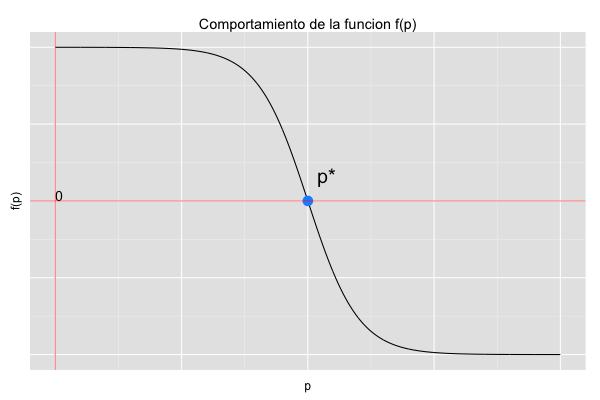
\includegraphics[width=1\textwidth]{Figures/Chapter2_fp}	
  \caption[Comportamiento de $f(\rho)$.]
  {La función $f(\rho)$ es no creciente para toda $\rho$. El valor de $f(\rho) = \lambda_{G(\rho)1}+ \lambda_{G(\rho)2} + ... +\lambda_{G(\rho)p}.$ $f(\rho^*) = 0 $}
\end{figure}


\begin{example} \label{ex:1}
Para ejemplificar el lema 1.4 se muestran las matrices $A,B \in {\rm I\!R}^{3 \times 3}$. Para el valor de $f(\rho)$ se utiliza la propiedad (1.29):

$$f(\rho) = \lambda_{G(\rho)1} + \lambda_{G(\rho)2} + ... + \lambda_{G(\rho)p}$$

con $p$ la dimensión a la que se va a proyectar. 


\begin{equation*}
A = \left(\!
    \begin{array}{ccc}
      4 & 0 & 0 \\
      0 & 6 & 0 \\
      0 & 0 & 8 
    \end{array}
  \!\right), \quad
B = \left(\!
    \begin{array}{ccc}
      1.5 & 0 & 0 \\
      0 & 2.5 & 0 \\
      0 & 0 & 5 
    \end{array}
\!\right) 
\end{equation*}



\begin{equation*}
G(\rho) = A- \rho B = \left(\!
    \begin{array}{ccc}
      4-1.5\rho & 0 & 0 \\
      0 & 6-2.5\rho & 0 \\
      0 & 0 & 8-5\rho 
    \end{array}   	
      \!\right) 
\end{equation*}

Los eigenvalores de esta matriz son $4-1.5\rho$,  $6-2.5\rho$ y  $8-5\rho$. Las funciones graficadas de estos eigenvalores se presentan en la figura 1.5.

\begin{figure}[!ht] \label{Fig1.4}
  \centering
  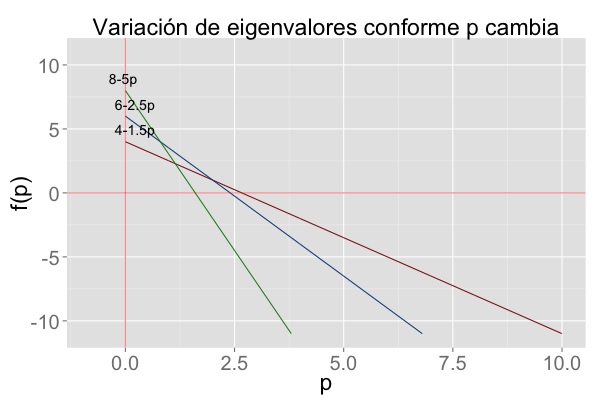
\includegraphics[width=1\textwidth]{Figures/Chapter2_3eigen}  
  \caption[Gráfica de los eigenvalores en función de $\rho$.] {Cada línea representa como se comporta cada eigenvalor de $A- \rho B$ cuando se varía $\rho$.}
\end{figure}

Cuando se desea que el proyector sea de dimensión 1, entonces se tiene que $f(\rho)$ es el eigenvalor más grande,  cuando sea de dimensión 2, la suma de los dos más grandes y así respectivamente. El valor de $f(\rho)$ para estos tres casos está representado en la figura 1.5.

\begin{figure}[!ht] \label{Fig1.5}
  \centering
  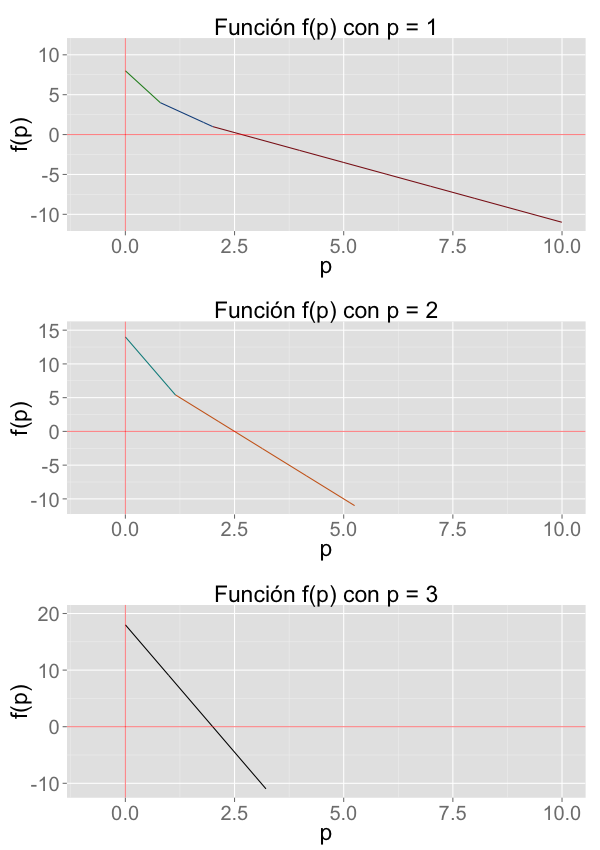
\includegraphics[width=1\textwidth]{Figures/Chapter2_grid3eigen}  
  \caption[$f(\rho)$ para proyectores de 1,2 y 3 dimensiones.] {La figura superior representa a $f(\rho) = \lambda_{G(\rho)_1}$, la de enmedio $f(\rho) = \lambda_{G(\rho)_1} + \lambda_{G(\rho)_2}$ y la de abajo $f(\rho) = \lambda_{G(\rho)_1} + \lambda_{G(\rho)_2} + \lambda_{G(\rho)_3}$.}
\end{figure}

\end{example}
\pagebreak

\subsection{Localización del óptimo}

En la sección anterior se encontró que la maximización al cociente de trazas puede ser visto como el problema de encontrar la raíz de la función $f(\rho) = max_{V^T V= I} Tr(V^T(A-\rho B)V)$. Por esto, encontrar un intervalo $(\rho_1, \rho_2)$ que contenga al valor óptimo $\rho^*$ puede reducir el número de iteraciones del método. Usando el lema 1.4 se sabe que $f$ es una función no creciente de $\rho$. Por esta razón si se encuentra una $\rho_1$ y $\rho_2$ tal que $f(\rho_1) \geq 0$ y $f(\rho_2) \leq 0$ y con la propiedad de continuidad de la funcion $f(\rho)$ entonces se encontró un intervalo que contiene a $\rho^*$. 

En esta tesis se dan cotas para el valor de $\rho^*$, la primera en función los eigenvalores de una transformación de $B -\rho A$ y la segunda en función de los eigenvalores de $B$ y $A$ \cite{ngo2012trace}. La demostración de cada una requiere del conocimiento del concepto de inercia y del Teorema de la Inercia de Sylvester. Por este motivo se presentan a continuación: \footnote{La demostración de este teorema puede ser encontrada en \cite{golub2012matrix}.}

\begin{definition}
La inercia de una matriz simétrica $A$ es la tripleta de enteros no negativos $(m, z, p)$ donde $m$, $z$ y $p$ son respectivamente el número de eigenvalores negativos, cero y positivos de $A$ \cite{golub2012matrix}.
\end{definition}

\begin{theorem}\label{teorem.2}
Sea $A \in {\rm I\!R}^{n \times n}$ una matriz simétrica y $Z \in {\rm I\!R}^{n \times n}$ no singular. Entonces $A$ y $Z^T A Z$ tienen la misma inercia \cite{golub2012matrix}.
\end{theorem}

\begin{proposition}
La raíz $\rho^*$ de $f(\rho)$ está localizada en el intervalo $(\lambda_p, \lambda_1)$ donde $\lambda_p$ es el p-ésimo eigenvalor más grande de $Z^T(A-\rho B)Z$.
\end{proposition}

\begin{proof}
Sea $Z$ la matriz que diagonaliza a $A-\rho B$ de manera que\footnote{El cálculo de esta matriz puede obtenerse en el algoritmo 8.7.1 de \cite{golub2012matrix}}:

\begin{equation}\label{eq:2.38}
\begin{aligned}
 Z^T AZ = \Lambda \\ Z^T B Z = I
 \end{aligned}
\end{equation}

Con $\Lambda$ una matriz diagonal y $\mu_1, \ldots,  \mu_n$ sus respectivos eigenvalores e $I$ la identidad de tamaño $n$. Entonces por el teorema 1.2 se sabe que $A- \rho B$ y $Z^T(A- \rho B)Z = \Lambda -\rho I$ tienen el mismo número de eigenvalores positivos, negativos y cero. Por lo tanto, la matriz en cuestión es de la siguiente forma:

\begin{equation}\label{eq:2.39}
\Lambda - \rho I = 
\left(\!
    \begin{array}{cccc}
      \mu_1 & 0 & \hdots & 0\\
      0 & \mu_2 & \hdots & 0\\
      \vdots & \vdots & \ddots & \vdots \\
      0 & 0 & \hdots & \mu_n
    \end{array}
  \!\right) - \rho
  \left(\!
    \begin{array}{cccc}
      1 & 0 & \hdots & 0\\
      0 & 1 & \hdots & 0\\
      \vdots & \vdots & \ddots & \vdots \\
      0 & 0 & \hdots & 1
    \end{array}
  \!\right) 
\end{equation} 

Como la  matriz $V$ de (1.9) es de tamaño $n \times p$, solo nos interesa saber el signo de los $p$ eigenvalores más grandes. Tomando $\rho = \mu_p$ entonces los elementos de la diagonal de la matriz $\Lambda- \rho I$ son de la forma:


\begin{equation}\label{eq:2.40}
\begin{aligned}
   \mu_i - \mu_p & \geq 0  \quad para \quad i \geq p\\
   \mu_i - \mu_p & \leq 0  \quad para \quad i \leq p
\end{aligned}
\end{equation} 

Los primeros p elementos tienen la propiedad de ser no negativos, ya que $\lambda_{(A-\rho B)_1} \geq \lambda_{(A-\rho B)_2} \geq ... \geq \lambda_{(A-\rho B)_p}$. Usando el teorema 1.2 se sabe que los primeros p eigenvalores de $A-\rho B$ también son no negativos. Por ende la suma de ellos es mayor o igual que cero. 

Por otro lado si se toma $\rho = \mu_1$. Entonces los elementos de la diagonal de la matriz (1.38) son de la forma:

\begin{equation}\label{eq:2.41}
   \mu_i - \mu_1  \leq 0 \quad \forall \quad i
\end{equation} 

Con $i = 1, ..., p$, cada uno de los elementos de la diagonal tiene la propiedad de ser no positivo por el mismo argumento que el caso pasado. Por lo tanto los $p$ eigenvalores más grandes de $\Lambda - \rho I$ y de $A-\rho B$ son no positivos, por lo que su suma es menor o igual que cero:

\begin{equation}\label{eq:2.42}
  \rho = \mu_p  \Rightarrow \sum_{i=1}^{p} (\mu_i- \mu_p) \geq 0 \Rightarrow f(\rho) \geq 0
\end{equation}

\begin{equation}\label{eq:2.43}
  \rho = \mu_1  \Rightarrow \sum_{i=1}^{p} (\mu_i - \mu_1) \leq 0 \Rightarrow f(\rho) \leq 0
\end{equation}

\end{proof}

\pagebreak

\begin{example} \label{ex:2}
Tomando las matrices A,B iguales que en el ejercicio 1.1, se puede encontrar fácilmente a la matriz $Z$:


\begin{equation*}
Z = \left(\!
    \begin{array}{ccc}
      \sqrt(\frac{1}{1.5}) & 0 & 0 \\
      0 & \sqrt(\frac{1}{2.5}) & 0 \\
      0 & 0 & \sqrt(\frac{1}{5}) 
    \end{array}
  \!\right)
\end{equation*}

Con la matriz $Z$ definida de esta manera, $Z^T A  Z = \Lambda$ y $Z^T B Z = I$ toman la siguiente forma:

\begin{equation*}
\Lambda - \rho I = 
\left(\!
    \begin{array}{ccc}
      \frac{4}{1.5} & 0  & 0\\
      0 & \frac{6}{2.5}  & 0\\
      0 & 0 & \frac{8}{5}
    \end{array}
  \!\right) - \rho
  \left(\!
    \begin{array}{ccc}
      1 & 0 & 0\\
      0 & 1 & 0\\
      0 & 0 & 1
    \end{array}
  \!\right) 
\end{equation*}

Entonces se puede encontrar un intervalo tal que $\rho^* \in \big[\rho_1, \rho_2 \big]$:

\begin{equation*}
  \begin{aligned}
\rho_1 &= \mu_p \\
\rho_2 &= \mu_1  
  \end{aligned}
\end{equation*}

Conforme el tamaño de la dimensión a proyectar cambia, las cotas son las siguientes:

\begin{equation*}
  \begin{aligned}
  p =& 1 \Rightarrow \qquad \rho_1 = \frac{4}{1.5} \quad y \quad \rho_2 = \frac{4}{1.5}\\
  p =& 2 \Rightarrow \qquad \rho_1 = \frac{4}{1.5} \quad y \quad \rho_2 = \frac{6}{2.5} \\
  p =& 3 \Rightarrow \qquad \rho_1 = \frac{4}{1.5} \quad y \quad \rho_2 = \frac{8}{5}
  \end{aligned}
\end{equation*}
 

 Estas cotas se pueden ver más fácil en la figura 1.6,donde se observa $f(\rho)$ con respecto a $p$:

\begin{figure}[!ht] \label{Fig1.6}
  \centering
  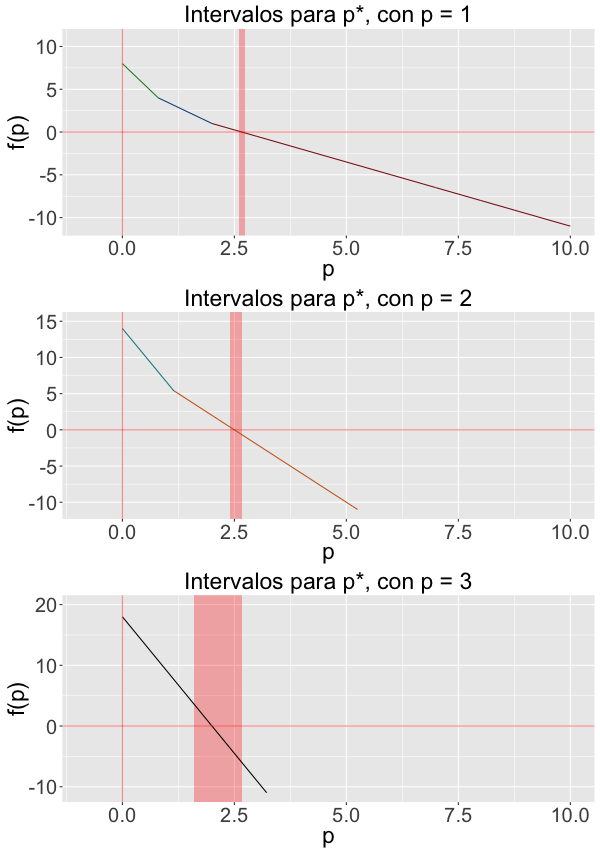
\includegraphics[width=.9\textwidth]{Figures/Chapter2_grid3eigen_interv}  
  \caption[Intervalos para $\rho^*$.] {La figura superior representa intervalos para $\rho^*$ cuando $f(\rho) = \lambda_{G(\rho)_1}$, la de enmedio cuando $f(\rho) = \lambda_{G(\rho)_1} + \lambda_{G(\rho)_2}$ y la de abajo cuando $f(\rho) = \lambda_{G(\rho)_1} + \lambda_{G(\rho)_2} + \lambda_{G(\rho)_3}$.}
\end{figure}

\end{example}

Otro intervalo que se ha desarrollado tiene que ver con directamente con los eigenvalores de $A$ y $B$ en lugar de los obtenidos por la matriz $A-\rho B$:

\pagebreak
\begin{proposition}
Sea $B$ positiva definida, entonces la raíz $\rho^*$ de $f(\rho)$ es tal que \cite{ngo2012trace}:

\begin{equation*}
\frac{\sum_{i = 1}^{p}\lambda_{A_i}}{\sum_{i = 1}^{p}\lambda_{B_i}} \leq \rho^* \leq \frac{\sum_{i = 1}^{p}\lambda_{(A)_i}}{\sum_{i = 1}^{p}\lambda_{(B)_{n-i+1}}}	
\end{equation*}

con $\lambda_{A_i}$ y $\lambda_{B_i}$ el i-ésimo eigenvalor más grande  de la matriz $A$ y $B$ respectivamente \cite{ngo2012trace}. 
\end{proposition}


\begin{proof}
Se tiene la propiedad que para una $p$ dada:


\begin{equation}\label{eq:2.44}
\max_{V^T V = I} Tr(V^T A V) =  Tr(V^{T*} A V^*) = \sum_{i=1}^p \lambda_{A_i }
\end{equation}
 
Con $\lambda_{A_i}$ los eigenvalores de A. Como esta $V^*$ maximiza la traza sobre $A$, entonces no necesariamente maximiza la de $B$. Al sustituirla en $Tr(V^{T} B V)$ se tiene que: 

\begin{equation}\label{eq:2.45}
Tr(V^{T*} B V^*) \leq \sum_{i=1}^p \lambda_{B_i }
\end{equation}

Con $\lambda_{B_i}$ los eigenvalores de B. Al hacer el cociente de (1.43) y (1.44) Se puede acotar inferiormente a $\rho^*$:


\begin{equation*}
  \frac{\sum_{i=1}^p \lambda_{A_i}} {\sum_{i=1}^p \lambda_{B_i}} \leq \frac{Tr(V^{T*} A V^*)}{Tr(V^{T*} B V^*)} \leq \max_{V^T V} \frac{Tr(V^{T} A V)}{Tr(V^{T} B V)} = \rho^*
\end{equation*}

Ahora falta acotarlo superiormente. Usando las siguientes propiedades que son derivadas de (1.27):

\begin{equation}\label{eq:2.46}
  Tr(V^T A V) \leq \sum_{i=1}^p \lambda_{A_i} 
\end{equation}

\begin{equation}\label{eq:2.47}
  Tr(V^T B V) \geq \sum_{i=1}^p \lambda_{B_{(n-i+1)}}
\end{equation}

La expresión (1.46) es la suma de los p eigenvalores más chicos de $B$. Dividiendo (1.45) entre (1.46) se tiene que para cualquier matriz ortogonal $V$:

\begin{equation}\label{eq:2.48}
   \frac{Tr(V^{T} A V)}{Tr(V^{T} B V)} \leq \frac{\sum_{i=1}^p \lambda_{A_i}}{\sum_{i=1}^p \lambda_{B_{(n-i+1)}}}
\end{equation}

En particular si se toma $V = V^{**}$ (La matriz con la que se alcanza $\rho^*)$:

\begin{equation}\label{eq:2.49}
  \rho^* = \frac{Tr(V^{T**} A V^{**})}{Tr(V^{T**} B V^{**})} \leq \frac{\sum_{i=1}^p \lambda_{A_i}}{\sum_{i=1}^p \lambda_{B_{(n-i+1)}}}
\end{equation}

\end{proof}
\begin{example}
Para ejemplificar esta cota se usará las matrices $A$ y $B$ de los dos ejemplos anteriores y se muestra en la figura 1.7.


\begin{equation*}
A = \left(\!
    \begin{array}{ccc}
      4 & 0 & 0 \\
      0 & 6 & 0 \\
      0 & 0 & 8 
    \end{array}
  \!\right), \quad
B = \left(\!
    \begin{array}{ccc}
      1.5 & 0 & 0 \\
      0 & 2.5 & 0 \\
      0 & 0 & 5 
    \end{array}
\!\right) 
\end{equation*}


(i) Para $p = 1$ la cota es la siguiente:
\begin{equation*}
\begin{aligned}
  \lambda_{A_1} = 8 \qquad
  \lambda_{B_1} = 5 \qquad
  \lambda_{B_3} = 1.5
\end{aligned}
\end{equation*}

\begin{equation*}
\begin{aligned}
\rho_1 = \frac{\sum_{i = 1}^{p}\lambda_{A_i}}{\sum_{i = 1}^{p}\lambda_{B_i}}  = \frac{8}{5} \qquad
\rho_2 = \frac{\sum_{i = 1}^{p}\lambda_{A_i}}{\sum_{i = 1}^{p}\lambda_{B_{n-i+1}}}  = \frac{8}{1.5}
\end{aligned}
\end{equation*}

(ii) Para $p = 2$ la cota es la siguiente:

\begin{equation*}
\begin{aligned}
\sum_{i = 1}^{2}\lambda_{A_1}  =& 14 \qquad
\sum_{i = 1}^{2}\lambda_{B_1}  =& 7.5 \qquad
\sum_{i = 1}^{2}\lambda_{B_{3-i+1}} =& 4
\end{aligned}
\end{equation*}

\begin{equation*}
\begin{aligned}
\rho_1 = \frac{\sum_{i = 1}^{p}\lambda_{A_i}}{\sum_{i = 1}^{p}\lambda_({B_i)}}
 = \frac{14}{7.5} \qquad
\rho_2 = \frac{\sum_{i = 1}^{p}\lambda_{A_i}}{\sum_{i = 1}^{p}\lambda_{B_{n-i+1}}}  = \frac{14}{4}
\end{aligned}
\end{equation*}



(iii) Para $p = 3$ la cota es la siguiente:
\begin{equation*}
  \begin{aligned}
  \sum_{i = 1}^{3}\lambda_{A_1}  = 18 \qquad
  \sum_{i = 1}^{3}\lambda_{B_1}  = 9 \qquad
  \sum_{i = 1}^{3}\lambda_{B_{n-i+1}}  = 9
  \end{aligned}
\end{equation*}

\begin{equation*}
  \begin{aligned}
\rho_1 = \frac{\sum_{i = 1}^{p}\lambda_{A_i}}{\sum_{i = 1}^{p}\lambda_{B_i}}  = \frac{18}{9} \qquad
\rho_2 = \frac{\sum_{i = 1}^{p}\lambda_{A_i}}{\sum_{i = 1}^{p}\lambda_{B_{n-i+1}}}  = \frac{18}{9}
  \end{aligned}
\end{equation*}

\end{example}

\begin{figure}[!ht] \label{Fig1.7}
  \centering
  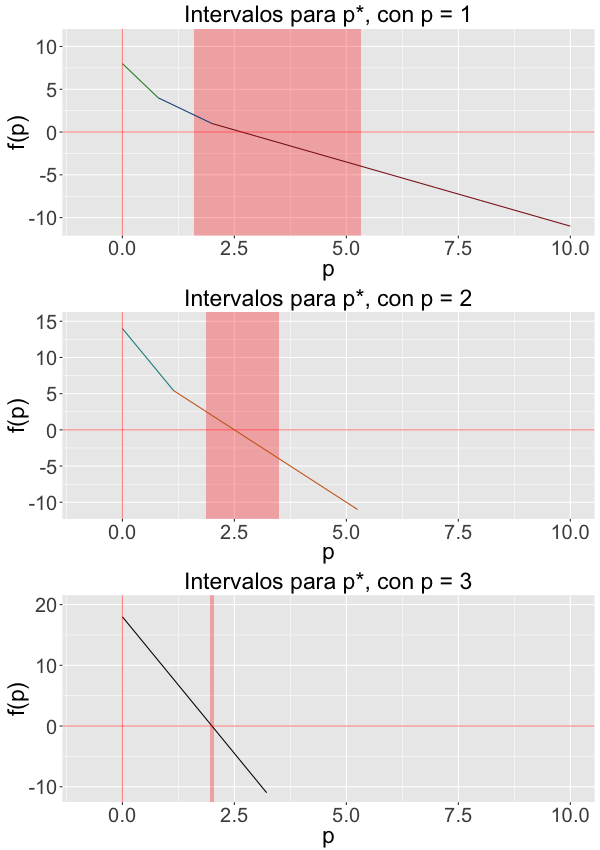
\includegraphics[width=.9 \textwidth]{Figures/Chapter2_grid3eigen_interv2}  
  \caption[Intervalos para $\rho^*$.] {La figura superior representa intervalos para $\rho^*$ cuando $f(\rho) = \lambda_{G(\rho)_1}$, la de enmedio cuando $f(\rho) = \lambda_{G(\rho)_1} + \lambda_{G(\rho)_2}$ y la de abajo cuando $f(\rho) = \lambda_{G(\rho)_1} + \lambda_{G(\rho)_2} + \lambda_{G(\rho)_3}$.}
\end{figure}



